\chapter{Other Dictionary Implementations}

AVL trees give $\Theta(\log n)$ worst case, but they are fiddly to implement and
use extra space for heights. This module looks at two alternatives: a
randomized structure (skip lists) that is easy to code with the same expected
bounds, and the idea of reordering items when the access pattern is not uniform.

\section{Skip Lists}

\begin{definition}
A \emph{skip list} is a hierarchy of sorted linked lists $S_0, S_1, \ldots, S_h$:
\begin{itemize}
  \item each list starts with a sentinel $-\infty$ and ends with $+\infty$;
  \item $S_0$ contains every key;
  \item each $S_{i+1}$ is a subset of $S_i$ (a key in $S_i$ is copied into
        $S_{i+1}$ with some probability, independently);
  \item $S_h$ contains only the sentinels.
\end{itemize}
Each node (a \emph{tower} element) has pointers \code{after} (next in the same
list) and \code{below} (same key in the list beneath).
\end{definition}

\begin{example}
\begin{verbatim}
S3: -inf ---------------------------------------- +inf
S2: -inf ------------- 37 ----------------------- +inf
S1: -inf ----- 23 ---- 37 ------------ 83 ------- +inf
S0: -inf - 10 - 23 - 31 - 37 - 44 - 65 - 83 - 92 - +inf
\end{verbatim}
\end{example}

Drawn as towers, with the search path for 65 in red: it ends at 44, the
predecessor of 65 in $S_0$, and 65 is the next key.
\begin{center}
\begin{tikzpicture}[sk/.style={draw,minimum width=8mm,minimum height=5mm,inner sep=1pt,font=\scriptsize}]
  \node[font=\scriptsize,anchor=east] at (-0.6,0.00) {$S_0$};
  \node[sk,fill=gray!15] (n0_0) at (0.00,0.00) {$-\infty$};
  \node[sk,fill=white] (n0_1) at (1.10,0.00) {10};
  \node[sk,fill=white] (n0_2) at (2.20,0.00) {23};
  \node[sk,fill=white] (n0_3) at (3.30,0.00) {31};
  \node[sk,fill=orange!25] (n0_4) at (4.40,0.00) {37};
  \node[sk,fill=orange!25] (n0_5) at (5.50,0.00) {44};
  \node[sk,fill=white] (n0_6) at (6.60,0.00) {65};
  \node[sk,fill=white] (n0_7) at (7.70,0.00) {83};
  \node[sk,fill=white] (n0_8) at (8.80,0.00) {92};
  \node[sk,fill=gray!15] (n0_9) at (9.90,0.00) {$+\infty$};
  \draw[-{Stealth}] (n0_0) -- (n0_1);
  \draw[-{Stealth}] (n0_1) -- (n0_2);
  \draw[-{Stealth}] (n0_2) -- (n0_3);
  \draw[-{Stealth}] (n0_3) -- (n0_4);
  \draw[-{Stealth}] (n0_4) -- (n0_5);
  \draw[-{Stealth}] (n0_5) -- (n0_6);
  \draw[-{Stealth}] (n0_6) -- (n0_7);
  \draw[-{Stealth}] (n0_7) -- (n0_8);
  \draw[-{Stealth}] (n0_8) -- (n0_9);
  \node[font=\scriptsize,anchor=east] at (-0.6,0.80) {$S_1$};
  \node[sk,fill=gray!15] (n1_0) at (0.00,0.80) {$-\infty$};
  \node[sk,fill=white] (n1_2) at (2.20,0.80) {23};
  \node[sk,fill=orange!25] (n1_4) at (4.40,0.80) {37};
  \node[sk,fill=white] (n1_7) at (7.70,0.80) {83};
  \node[sk,fill=gray!15] (n1_9) at (9.90,0.80) {$+\infty$};
  \draw[-{Stealth}] (n1_0) -- (n1_2);
  \draw[-{Stealth}] (n1_2) -- (n1_4);
  \draw[-{Stealth}] (n1_4) -- (n1_7);
  \draw[-{Stealth}] (n1_7) -- (n1_9);
  \draw[gray] (n1_0) -- (n0_0);
  \draw[gray] (n1_2) -- (n0_2);
  \draw[gray] (n1_4) -- (n0_4);
  \draw[gray] (n1_7) -- (n0_7);
  \draw[gray] (n1_9) -- (n0_9);
  \node[font=\scriptsize,anchor=east] at (-0.6,1.60) {$S_2$};
  \node[sk,fill=orange!25] (n2_0) at (0.00,1.60) {$-\infty$};
  \node[sk,fill=orange!25] (n2_4) at (4.40,1.60) {37};
  \node[sk,fill=gray!15] (n2_9) at (9.90,1.60) {$+\infty$};
  \draw[-{Stealth}] (n2_0) -- (n2_4);
  \draw[-{Stealth}] (n2_4) -- (n2_9);
  \draw[gray] (n2_0) -- (n1_0);
  \draw[gray] (n2_4) -- (n1_4);
  \draw[gray] (n2_9) -- (n1_9);
  \node[font=\scriptsize,anchor=east] at (-0.6,2.40) {$S_3$};
  \node[sk,fill=orange!25] (n3_0) at (0.00,2.40) {$-\infty$};
  \node[sk,fill=gray!15] (n3_9) at (9.90,2.40) {$+\infty$};
  \draw[-{Stealth}] (n3_0) -- (n3_9);
  \draw[gray] (n3_0) -- (n2_0);
  \draw[gray] (n3_9) -- (n2_9);
  \draw[-{Stealth},very thick,red!70!black,shorten <=1pt,shorten >=1pt] ($(n3_0)+(0.15,-0.27)$) -- ($(n2_0)+(0.15,0.27)$);
  \draw[-{Stealth},very thick,red!70!black,shorten <=1pt,shorten >=1pt] ($(n2_0)+(0.42,0.13)$) -- ($(n2_4)+(-0.42,0.13)$);
  \draw[-{Stealth},very thick,red!70!black,shorten <=1pt,shorten >=1pt] ($(n2_4)+(0.15,-0.27)$) -- ($(n1_4)+(0.15,0.27)$);
  \draw[-{Stealth},very thick,red!70!black,shorten <=1pt,shorten >=1pt] ($(n1_4)+(0.15,-0.27)$) -- ($(n0_4)+(0.15,0.27)$);
  \draw[-{Stealth},very thick,red!70!black,shorten <=1pt,shorten >=1pt] ($(n0_4)+(0.42,0.13)$) -- ($(n0_5)+(-0.42,0.13)$);
\end{tikzpicture}
\end{center}

\subsection{Search}

Start at the top-left sentinel. Move right while the next key is smaller than
$k$; otherwise drop down. Record the path (the last node visited on each level)
because insert and delete need it.
\begin{lstlisting}
get-predecessors(k):
  p <- topmost left sentinel
  P <- empty stack
  P.push(p)
  while p.below != nil do
    p <- p.below
    while p.after.key < k do p <- p.after
    P.push(p)
  return P                     // P.top() is the predecessor of k in S0

skip-search(L, k):
  P <- get-predecessors(k)
  p0 <- P.top()
  if p0.after.key = k then return p0.after
  else return "not found"
\end{lstlisting}

\subsection{Insert}

Flip a fair coin until tails; if we got $i$ heads, the new key goes into lists
$S_0, \ldots, S_i$. If $i \ge h$, first add new empty levels so that the top
list stays sentinel-only. Then splice the key in after each predecessor in the
stack $P$, from bottom up, linking \code{below} pointers.

\begin{lstlisting}
skip-insert(L, k, v):
  i <- 0
  while random(2) = 1 do i <- i + 1     // tower height
  while height(L) <= i do add a new empty top level
  P <- get-predecessors(k)
  below <- nil
  for level <- 0 to i do
    p <- P.pop()                         // predecessor on this level
    z <- new node (k, v) with z.below <- below
    z.after <- p.after; p.after <- z
    below <- z
\end{lstlisting}

\subsection{Delete}

Find the predecessors, then on each level where \code{p.after.key = k}, unlink
it. Afterwards remove extra empty top lists so only one sentinel-only list remains.

\subsection{Analysis}

Let tower heights be geometric: $\Pr[\text{height} \ge i] = 2^{-i}$.
\begin{itemize}
  \item \textbf{Space.} Expected list sizes: $\mathbb E|S_i| = n/2^i$, so the
        expected total number of nodes is $\sum_i n/2^i = 2n \in \bigO(n)$.
  \item \textbf{Height.} $\Pr[\text{some tower has height} \ge i] \le n/2^i$.
        With $i = 3\log n$ this is $\le 1/n^2$, so the height is $\bigO(\log n)$
        with high probability; expected height $\le \log n + 2$.
  \item \textbf{Search time.} Count drop-downs plus forward steps. Drop-downs are
        the height. Analyse the search path backward: from a node at level $\ell$,
        we came from the left (a scan step) if the node's tower stops at $\ell$,
        or from above if it continues --- each with probability $1/2$. So the
        expected number of scan steps per level is at most 1, giving expected
        search time $\bigO(\log n)$.
\end{itemize}

\begin{center}
\begin{tabular}{lll}
\toprule
Operation & Expected & Worst case\\
\midrule
\code{search}, \code{insert}, \code{delete} & $\bigO(\log n)$ & unbounded / $\Theta(n)$ per level\\
space & $\bigO(n)$ & unbounded\\
\bottomrule
\end{tabular}
\end{center}

Skip lists are simple, need no rotations, and are used in practice (e.g.\ in
concurrent data structures). Their bounds are \emph{expected}: the randomness is
in the coin flips, not in the input.

\section{Re-ordering Items}

So far every key was assumed equally likely to be accessed. In practice accesses
are skewed (the 80/20 rule): a few items are requested most of the time. If we
store items in an unsorted list/array, placing popular items near the front
pays off.

\subsection{Optimal Static Ordering}

Suppose we know the access probabilities $p_1, \ldots, p_n$ of the items and do
not change the list. Accessing the item at position $i$ (1-indexed) costs $i$
comparisons. The expected search cost of an ordering is
\[
C = \sum_{i=1}^n i \cdot p_{(i)},
\]
where $p_{(i)}$ is the probability of the item at position $i$.

\begin{theorem}
The expected cost is minimised by sorting items in non-increasing order of
access probability.
\end{theorem}
\begin{proof}
Exchange argument: if positions $i < j$ hold items with $p_{(i)} < p_{(j)}$,
swapping them changes the cost by
$(i p_{(j)} + j p_{(i)}) - (i p_{(i)} + j p_{(j)}) = (j - i)(p_{(i)} - p_{(j)}) < 0$.
So any optimal ordering has no such inversions.
\end{proof}

\begin{example}
Keys A, B, C, D, E with probabilities $\frac2{20}, \frac8{20}, \frac1{20},
\frac{4}{20}, \frac{5}{20}$. In the given order, the expected cost is
$\frac{1\cdot 2 + 2\cdot 8 + 3 \cdot 1 + 4 \cdot 4 + 5\cdot 5}{20} = \frac{62}{20} = 3.1$.
In the optimal order B, E, D, A, C it is
$\frac{8 + 10 + 12 + 8 + 5}{20} = \frac{43}{20} = 2.15$.
\end{example}

\subsection{Dynamic Ordering: Move-To-Front and Transpose}

When probabilities are unknown or change over time, use a self-adjusting
heuristic.

\begin{itemize}
  \item \textbf{Move-To-Front (MTF):} after a successful search, move the found
        item to the front of the list. Insert new items at the front.
  \item \textbf{Transpose:} after a successful search, swap the found item with
        the item immediately before it.
\end{itemize}

\begin{lstlisting}
MTF-search(L, k):
  find k at position i by linear scan     // cost i
  if found then remove it and insert it at the front
\end{lstlisting}

MTF works well for a linked list (moving is $\Theta(1)$ once found); in an array
it costs $\Theta(i)$ to shift, which is the same order as the search, so it is
fine. Transpose is natural for arrays.

\paragraph{Comparison.}
\begin{itemize}
  \item MTF adapts quickly to changes in the access pattern (temporal locality),
        but one access to a rare item moves it to the front.
  \item Transpose changes slowly and is more stable, but has bad worst cases: two
        items at the back that are accessed alternately just swap with each
        other forever, each access costing $\Theta(n)$.
  \item MTF is \emph{2-competitive}: its total cost on any access sequence is at
        most twice that of the optimal static ordering (for that sequence) plus
        lower-order terms. Transpose has no such guarantee.
\end{itemize}

\begin{example}
List $[A, B, C, D, E]$, accesses D, D, B, D.
\begin{itemize}
  \item MTF: D (cost 4) gives $[D,A,B,C,E]$; D (1); B (3) gives $[B,D,A,C,E]$;
        D (2). Total 10.
\begin{center}
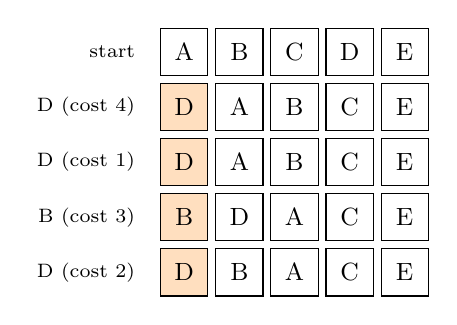
\begin{tikzpicture}[mt/.style={draw,minimum size=6mm,font=\small}]
  \node[mt,fill=white] at (0.0,0.0) {A};
  \node[mt,fill=white] at (0.7,0.0) {B};
  \node[mt,fill=white] at (1.4,0.0) {C};
  \node[mt,fill=white] at (2.1,0.0) {D};
  \node[mt,fill=white] at (2.8,0.0) {E};
  \node[font=\scriptsize,anchor=east] at (-0.5,0.0) {start};
  \node[mt,fill=orange!25] at (0.0,-0.7) {D};
  \node[mt,fill=white] at (0.7,-0.7) {A};
  \node[mt,fill=white] at (1.4,-0.7) {B};
  \node[mt,fill=white] at (2.1,-0.7) {C};
  \node[mt,fill=white] at (2.8,-0.7) {E};
  \node[font=\scriptsize,anchor=east] at (-0.5,-0.7) {D (cost 4)};
  \node[mt,fill=orange!25] at (0.0,-1.4) {D};
  \node[mt,fill=white] at (0.7,-1.4) {A};
  \node[mt,fill=white] at (1.4,-1.4) {B};
  \node[mt,fill=white] at (2.1,-1.4) {C};
  \node[mt,fill=white] at (2.8,-1.4) {E};
  \node[font=\scriptsize,anchor=east] at (-0.5,-1.4) {D (cost 1)};
  \node[mt,fill=orange!25] at (0.0,-2.1) {B};
  \node[mt,fill=white] at (0.7,-2.1) {D};
  \node[mt,fill=white] at (1.4,-2.1) {A};
  \node[mt,fill=white] at (2.1,-2.1) {C};
  \node[mt,fill=white] at (2.8,-2.1) {E};
  \node[font=\scriptsize,anchor=east] at (-0.5,-2.1) {B (cost 3)};
  \node[mt,fill=orange!25] at (0.0,-2.8) {D};
  \node[mt,fill=white] at (0.7,-2.8) {B};
  \node[mt,fill=white] at (1.4,-2.8) {A};
  \node[mt,fill=white] at (2.1,-2.8) {C};
  \node[mt,fill=white] at (2.8,-2.8) {E};
  \node[font=\scriptsize,anchor=east] at (-0.5,-2.8) {D (cost 2)};
\end{tikzpicture}
\end{center}
  \item Transpose: D (4) gives $[A,B,D,C,E]$; D (3) gives $[A,D,B,C,E]$;
        B (3) gives $[A,B,D,C,E]$; D (3). Total 13.
\end{itemize}
\end{example}

\begin{aside}
The same MTF idea reappears in Chapter 10 as a compression transform: frequently
recurring symbols get small indices.
\end{aside}

\section{Summary}
\begin{itemize}
  \item Skip lists: towers of geometric height; expected $\bigO(n)$ space and
        $\bigO(\log n)$ search/insert/delete; simple to implement.
  \item With known access probabilities, the best static unsorted order is by
        decreasing probability (exchange argument).
  \item With unknown probabilities, self-adjusting lists: MTF (2-competitive,
        adapts fast) or Transpose (conservative, bad worst case).
\end{itemize}
